\documentclass[12pt,a4paper]{univention}
\usepackage[utf8]{inputenc}
\usepackage[T1]{fontenc}
\usepackage{amsmath}
\usepackage{amsfonts}
\usepackage{float}
\usepackage{amssymb}
\usepackage{graphicx}
\author{Julia Bremer}
\setcounter{tocdepth}{3}
\usepackage[T1]{fontenc}
\usepackage{underscore}
\begin{document}

\maketitle{Mechanics of User Identification and Authentication}{Julia Bremer}{}{}
\tableofcontents
\newpage
\section{User Identification and Authentication Concepts}
\section{UNIX User Authentication Architeture}
\section{Windows User Authentication Architecture}
\section{Authentication Access to Services and Applications}
\subsection{SAML, WS-Security and Federated Identitiy}
\subsubsection{SAML}
The SAML standart allows organizations to establish trust relationships with another and with their customers.
This way, they can share resources with one another in a secure, trusted fashion. As a result, users can access resources of organizations in this trust relationship without having to authenticate with each one. To access a Service (Service Provider SP), they only need to authenticate against a central, trusted party, the IdP (Identity Provider). \\
The "identity provider" (IdP) is the SAML authentication authority, where the users account information is stored.\\
The "service providers" (SPs) have resources, such as Web servers, media servers, databases, etc. They may have their own local accounts, that have meaning only for the SP itself.\\
SPs trust their IdP to authenticate users. The IdP does not necessarily trusts the SPs.  
After authenticating, the user will be given an access token or Identity Provider  statement (called SAML assertion). The SAML assertion is an XML formatted structure that may contain:
\begin{itemize}
 \item \textit{User authentication information}. The assertion contains information, that proves the users successfull authentication. It also contains a typestamp and type of information etc
 \item \textit{Authorization information}. The assertion may contain information about the permissions of the user, e.g. which resources they have access to.
 \item \textit{Attributes} The assertion may contain attributes, such as the users e-mail address, telephone number, etc.
 \end{itemize} 
 The SAML specification relies on XML encryption and signing mechanisms to protect SAML messages from improper modification, and potentially from disclosure.\\
To provide for encryption and signing, XML can user asymmetric cryptography (often based on X.509 certificates) or symmetric keys, while certificate-based protection is the preferred approach.\\
SAML assertions are signed by the authentication authority that has issued them. SPs can verify the authentication by a trusted IdP by verifying this signature. The IdP needs to be trusted by all SPs for SAML to work.\\
Since SAML communication typically happens over HTTP it can be encapsulated within TLS/SSL (HTTPS).\\
\subsubsection{SAML and Web Single Sign-On}
In a Web single sign-on scenario, the user needs to authenticate first by providing a set of acceptable and correct credentials to the identity provider. Once the user has been authenticated, the web browser will optain the SAML assertion for the user, which at this stage is similar to a service ticket.\\
The user can connect to the Service Provider by presenting the signed SAML assertion. If the Service Provider can verify that the assertion is signed by a trusted Identity Provider, it can use the information in the security assertion to link the user to a local account and provide the user with access to local resources.\\
Once the user has obtained the SAML assertion, they can access resources from every other Service Provider that trusts the Identity Provider without having to re-authenticate.\\
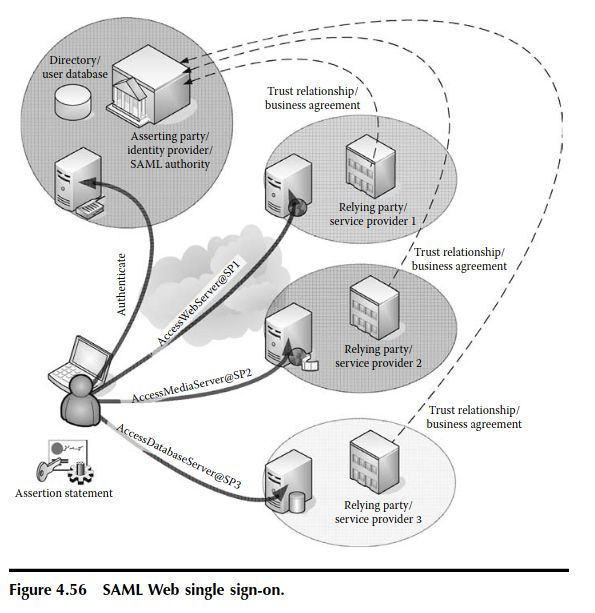
\includegraphics[scale=0.7]{samlauth.png}\\
\subsubsection{Case Study: Web Single Sign-On Mechanics}
\paragraph{Service Provider Redirect/POST Binding}
In this scenario, the user has not been authenticated yet. He tries to access a service provider with his browser. Since he has no SAML assertion yet, the Web server redirects the user to the Identity Providers authentication web page. The SP inserts the referring URL from the SP Web site in the redirection request.\\
After the user provided his credentials, the IdP generates a SAML assertion which is provided to the users Web browser.\\
It is important to note, that the user cannot modify the SAML assertion, since it is signed by the IdP and the user does not have the IdPs private key to generate a new signature.
\paragraph{Provider POST/Artifact Binding}
In this scenario, a user has not been authenticated yet and tries to access a Service Provider using his Web browser.\\
The Service Provider SAML service generates an artifact (reference) for the user request and returns it to the Web browser, along with a redirect to the Identity Provider. \\
The IdP uses synchrnous SOAP communication to connect directly to the service provider, resolves the artifact and \textbf{provides a security assertion to the sevice provider.}
The client is not involved in the SAML assertion submission process.\\
\paragraph{Identity Provider POST Binding}
In this scenario, the user access the identity provider first, authenticates and receives a SAML assertion. The user then can use a link on the IdPs Web site, that points to the Service Provider and submits the SAML assertion, that he already has.\\
\subsubsection{SAML Federated Identity}
The \textit{federated identity} use case is primarily meant for business-to-business communication. With this model, two or more partner organizations can federate their authentication authorities and allow useres from one organization to access resources in another organization using their own user accounts and credentials.\\
When a user in a federated identity model authenticates to his authentication authority, he is provided with a SAML assertion. This security assertion can then be used by the user to access resources in another domain in the SAML federation to which the user has been granted access.
\subsubsection{Account Linking}
\subsubsection{WS-Linking}


\section{Authentication Access to the Infrastructure}

\end{document}
